\chapter{Infinitary Term Rewriting}\label{chap:rewriting}

Before formally introducing term rewriting, we give an example of an
infinitary TRS taken from \citet{klop-de-vrijer-05} and trust the
reader to pick up the general ideas.

Let $A$, $B$ and $P$ be symbols with arities $0$, $1$ and $2$,
respectively. We consider the system consisting of the following rule:
\begin{align*}
A \rightarrow B(A)
\end{align*}
The term $A$
rewrites to $B(B(B(A)))$, written $B^3(A)$, in $3$ steps, or more
generally to $B^n(A)$ in $n$ steps for every $n \in \mathbb{N}$.
%\begin{align*}
%  A \rightarrow B(A) \rightarrow B(B(A)) \rightarrow \cdots \mbox{($n$
%    steps)} \cdots \rightarrow B^n(A)
%\end{align*}
\begin{center}
{\footnotesize\begin{tikzpicture}[node distance=50pt]
\tikzstyle{level}=[level distance=20pt,sibling distance=22pt]
\node (a) {$A$};
\node (b) [right of=a] {$B$} child { node {$A$} };
\node (c) [right of=b] {$B$} child { node {$B$} child { node {$A$} } };
\node (d) [right of=c] {$B$} child { node {$B$} child { node {$B$}
    child { node {$A$} } } };
\path (a) -- (b) node[midway,below=-1pt] {$\rightarrow$};
\path (b) -- (c) node[midway,below=-1pt] {$\rightarrow$};
\path (c) -- (d) node[midway,below=-1pt] {$\rightarrow$};
\end{tikzpicture}}
\end{center}\vspace{-0.8\baselineskip}
In the finitary setting, these are the only rewrite sequences from $A$
and all of them allow an additional step. Hence, $A$ has no normal
form.

The limit of these rewrite sequences, although non-existent in
finitary rewriting, is intuitively well-defined. It is reached in
$\omega$ many rewrite steps and we denote it by $B^\omega$. Infinitary
rewriting allows \begin{inparaenum}[(i)]
  \item infinite terms such as $B^\omega$ and
  \item rewrite sequences of transfinite length such as $A
    \rightarrow^\omega B^\omega$.
\end{inparaenum}\nopagebreak[3]
\begin{center}
{\footnotesize\begin{tikzpicture}[node distance=50pt]
\tikzstyle{level}=[level distance=20pt,sibling distance=22pt]
\node (a) {$A$};
\node (b) [right of=a] {$B$} child { node {$A$} };
\node (c) [right of=b] {$B$} child { node {$B$} child { node {$A$} } };
\node (d) [right of=c,node distance=80pt] {$B$} child { node {$B$} child { node {$B$}
    child { node[below=-6pt] {\scriptsize$\vdots$} } } };
\path (a) -- (b) node[midway,below=-1pt] {$\rightarrow$};
\path (b) -- (c) node[midway,below=-1pt] {$\rightarrow$};
\path (c) -- (d) node[midway,below=-1pt] {$\rightarrow \quad \cdots$};
\end{tikzpicture}}
\end{center}\vspace{-0.8\baselineskip}
The word `transfinite' hints that there are also rewrite sequences of
length $> \omega$. Consider for example the term $P(A, A)$. We can
rewrite this term to $P(B^\omega, A)$ in $\omega$ many steps, and
rewrite $P(B^\omega, A)$ to $P(B^\omega, B^\omega)$ in another
$\omega$ many steps. Therefore we have $P(A, A) \rightarrow^{\omega
  \times 2} P(B^\omega, B^\omega)$.
\begin{center}
{\footnotesize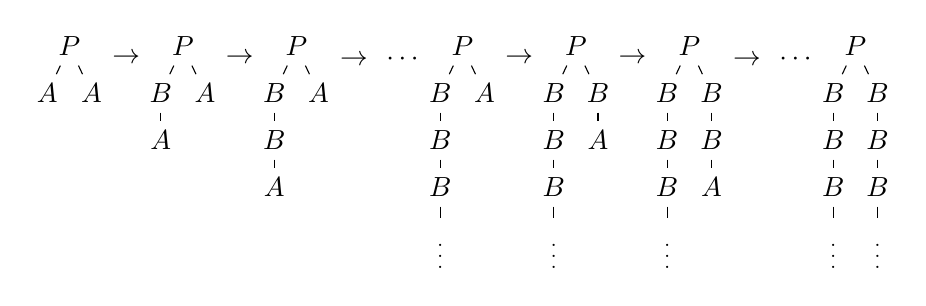
\begin{tikzpicture}[node distance=41pt]
\tikzstyle{level}=[level distance=17pt,sibling distance=16pt]
\node (a) {$P$} child { node {$A$} } child { node {$A$} };
\node (b) [right of=a] {$P$} child { node {$B$} child { node {$A$} } } child { node {$A$} };
\node (c) [right of=b] {$P$} child { node {$B$} child { node {$B$}
    child { node {$A$} } } } child { node {$A$} };
\node (d) [right of=c,node distance=60pt] {$P$} child { node {$B$} child { node {$B$}
    child { node {$B$} child { node[below=-6pt] {\scriptsize$\vdots$} } } } } child { node {$A$} };
\node (e) [right of=d] {$P$} child { node {$B$} child { node {$B$}
    child { node {$B$} child { node[below=-6pt] {\scriptsize$\vdots$} } } } }
child { node {$B$} child { node {$A$} } };
\node (f) [right of=e] {$P$} child { node {$B$} child { node {$B$}
    child { node {$B$} child { node[below=-6pt] {\scriptsize$\vdots$} } } } }
child { node {$B$} child { node {$B$} child { node {$A$} } } };
\node (g) [right of=f,node distance=60pt] {$P$} child { node {$B$} child { node {$B$}
    child { node {$B$} child { node[below=-6pt] {\scriptsize$\vdots$} } } } }
child { node {$B$} child { node {$B$} child { node {$B$} child {
        node[below=-6pt] {\scriptsize$\vdots$} } } } };
\path (a) -- (b) node[midway,below=-1pt] {$\rightarrow$};
\path (b) -- (c) node[midway,below=-1pt] {$\rightarrow$};
\path (c) -- (d) node[midway,below=-1pt] {$\rightarrow \, \: \cdots$};
\path (d) -- (e) node[midway,below=-1pt] {$\rightarrow$};
\path (e) -- (f) node[midway,below=-1pt] {$\rightarrow$};
\path (f) -- (g) node[midway,below=-1pt] {$\rightarrow \, \: \cdots$};
\end{tikzpicture}}
\end{center}\vspace{-0.8\baselineskip}
However, $P(B^\omega, B^\omega)$ can also be reached from $P(A, A)$ in
$\omega$ many steps, alternating the steps from the two $\omega$-step
rewrite sequences.
\begin{center}
{\footnotesize\begin{tikzpicture}[node distance=50pt]
\tikzstyle{level}=[level distance=20pt,sibling distance=22pt]
\node (a) {$P$} child { node {$A$} } child { node {$A$} };
\node (b) [right of=a] {$P$} child { node {$B$} child { node {$A$} } } child { node {$A$} };
\node (c) [right of=b] {$P$} child { node {$B$} child { node {$A$} } }
child { node {$B$} child { node {$A$} } };
\node (d) [right of=c] {$P$} child { node {$B$} child { node {$B$}
    child { node {$A$} } } }
child { node {$B$} child { node {$A$} } };
\node (e) [right of=d] {$P$} child { node {$B$} child { node {$B$}
    child { node {$A$} } } }
child { node {$B$} child { node {$B$} child { node {$A$} } } };
\node (f) [right of=e,node distance=80pt] {$P$} child { node {$B$} child { node {$B$}
    child { node {$B$} child { node[below=-6pt] {\scriptsize$\vdots$} } } } }
child { node {$B$} child { node {$B$} child { node {$B$} child {
        node[below=-6pt] {\scriptsize$\vdots$} } } } };
\path (a) -- (b) node[midway,below=-1pt] {$\rightarrow$};
\path (b) -- (c) node[midway,below=-1pt] {$\rightarrow$};
\path (c) -- (d) node[midway,below=-1pt] {$\rightarrow$};
\path (d) -- (e) node[midway,below=-1pt] {$\rightarrow$};
\path (e) -- (f) node[midway,below=-1pt] {$\rightarrow \quad \cdots$};
\end{tikzpicture}}
\end{center}\vspace{-0.8\baselineskip}
This observation is generalised in the Compression Lemma
(page~\pageref{lem:compression}).

In the following sections, we introduce the ordinal numbers and a
representation for them known as tree ordinals, and we present the
basic notions from the theory of term rewriting as required in the
following chapters.
% None of this is original material.

%This chapter does not contain original material. The construction of the
%order relation on tree ordinals in Section~\ref{sub:tree} is by
%\citet{hancock-08}.

% finitary rewriting: TRS as a programming language, or in theorem
% provers

% nonterminating processes, stream-based programming languages

% TODO: Short motivation for term rewriting, summation of its applications and
% aspects of rewriting that are studied.

%It should be noted that an infinite term is to be understood as a term
%with a \emph{possibly} infinite depth, that is, the class of infinite
%terms includes the finite terms.

%Orthogonal TRSs have some nice properties, for example UN$^{\infty}$ and
%compression.


\section{Ordinal Numbers}\label{sec:ordinals}

Ordinal numbers \citep{cantor-15}, or ordinals for short, are an
extension of the natural numbers with transfinite objects. Indeed, the
finite ordinals are just the natural numbers. The smallest infinite
ordinal is called $\omega$ and following $\omega$ we have $\omega +
1$, $\omega + 2$, \ldots, $\omega \times 2$. Then there are the
ordinals $\omega \times 2 + 1$, $\omega \times 2 + 2$, \ldots, $\omega
\times 3$. Some other (still relatively small) ordinals are:
\begin{displaymath}
  \omega^2 \qquad
  \omega^\omega \qquad
  \omega^{\omega^2} \qquad
  \omega^{\omega^\omega} \qquad
  \omega^{\omega^{\omega^{\iddots}}} = \epsilon_0
\end{displaymath}
Note that this is all merely notation, we have not yet defined a
representation for ordinals or what $+$, $\times$ and superscripts
are.

In set theory, ordinals are usually represented by hereditarily transitive
sets. Zero corresponds to the empty set $\nothing$, one to the
singleton $\{ \nothing \}$ and so on, and $\omega$ is represented by
$\{ \nothing, \{ \nothing \}, \{ \nothing, \{ \nothing \} \} , \ldots
\}$. Now $\in$ constitutes a well-founded total order on the
ordinals.

We abbreviate $\alpha \cup \{ \alpha \}$ by $\alpha^+$ and say that
$\alpha$ is a \emph{successor ordinal} if $\alpha = \beta^+$ for some
ordinal $\beta$. If $\alpha$ is not a successor ordinal and $\alpha
\neq \nothing$, it is called a \emph{limit ordinal}. Hence, an ordinal
can be either zero, a successor ordinal, or a limit ordinal.

%From now on, we make no distinction between an ordinal and its
%set-theoretic representation (e.g.\ between $0$ and $\nothing$).
Examples of successor ordinals are $4$, $\omega + 7$  and
$\omega^{\omega \times 2} + 1$. Examples of limit ordinals are
$\omega$ and $\omega \times 3$. Henceforth we use $\alpha, \beta,
\gamma, \lambda$ to denote ordinals where $\lambda$ always denotes a
limit ordinal.

One can do arithmetic on ordinals much like we do arithmetics on natural
numbers. For example, addition can be defined by recursion on the right
argument:
\begin{align*}
  \alpha + 0       &= \alpha\\
  \alpha + \beta^+ &= (\alpha + \beta)^+\\
  \alpha + \lambda &= \bigcup \{ \alpha + \gamma \; | \; \gamma \in \lambda \}
\end{align*}


\subsection{Tree Ordinals}\label{sub:tree}

% Possible reference for Brouwer ordinals:
% Constructivism in Mathematics: An Introduction, A.S. Troelstra en Dirk
% van Dalen, North-Holland Publishing, Amsterdam, 1988.

% Possible reference for Brouwer ordinals:
% Combinators, Lambda-Terms and Proof Theory, S. Stenlund, 1972

% Possible reference for Brouwer ordinals, Brouwer's Phd thesis:
% http://poortman.kb.nl/long2.php?TABEL=T_TITEL&ID=36516
% L. E. J. Brouwer en de grondslagen van de wiskunde
% Bewerkt door Dirk van Dalen, 2001
% ISBN 9050410618
%
% Structure of 'Brouwer ordinals' should have been in an early draft
% of this thesis and might be found in the annotated version.

% Reference for tree ordinals:
% Subrecursive hierarchies via direct limits, E.C. Dennis-Jones and
% S.S. Wainer
%
% See also Hydra Games and Tree Ordinals (Ariya Isihara)

The tree ordinals \citep{dennis-jones-wainer-84} are a representation
of the countable ordinals as countably branching well-founded
trees. Their inductive definition uses constructors $0$ (zero), $^+$
(successor) and $\sqcup$ (limit).

% Be alerted that all ordinals cannot form a set (only a class), but we are
% defining a subset here
\begin{definition}\label{def:ordinals}%[Ordinals]
The set of \emph{tree ordinals} $\Ord$ is defined by induction:
\begin{compactenum}
  \item
    $0 \in \Ord$.
  \item
    If $\alpha \in \Ord$, then $\alpha^+ \in \Ord$.
  \item
    If $\alpha_i \in \Ord$ for all $i \in \mathbb{N}$, then $\sqcup_i
    \alpha_i \in \Ord$.
\end{compactenum}
\end{definition}
The $\sqcup$ constructor has type $(\mathbb{N} \rightarrow \Ord) \rightarrow
\Ord$. For our convenience we write $\sqcup_i \cdots i \cdots$ instead
of $\sqcup (\lambda i . \cdots i \cdots)$. Sometimes we explicitly enumerate
the argument, writing for example $\sqcup \{ \alpha_1, \alpha_2,
\alpha_3, \ldots \}$.
% or: we write $\sqcup_i (f i)$ instead of $\sqcup_i f$

% TODO: make this a nice picture
\begin{figure}
\begin{center}
\begin{tikzpicture}[scale=0.9]
\tikzstyle{level 1}=[level distance=0cm, sibling distance=3cm]
\tikzstyle{level 2}=[level distance=0.8cm, sibling distance=3cm]
\tikzstyle{level 3}=[level distance=0.8cm, sibling distance=3cm]
\tikzstyle{level 4}=[level distance=1.5cm, sibling distance=3cm]
\tikzstyle{level 5}=[level distance=0.8cm, sibling distance=0.7cm]
\tikzstyle{level 6}=[level distance=0.8cm, sibling distance=0.7cm]
\tikzstyle{level 7}=[level distance=0.8cm, sibling distance=0.7cm]
\tikzstyle{level 8}=[level distance=0.8cm, sibling distance=0.7cm]

\coordinate
child {
  [fill] circle (1.5pt) edge from parent
child {
  [fill] circle (1.5pt) edge from parent
child {
 edge from parent
child {
  child {
    circle (1.5pt) edge from parent
  }
  child {
    [fill] circle (1.5pt)
    child {
      circle (1.5pt) edge from parent
    }
    edge from parent
  }
  child {
    [fill] circle (1.5pt)
    child {
      [fill] circle (1.5pt)
      child {
        circle (1.5pt) edge from parent
      }
      edge from parent
    }
    edge from parent
  }
  child {
    [fill] circle (1.5pt)
    child {
      [fill] circle (1.5pt)
       child {
        [fill] circle (1.5pt)
         child {
           circle (1.5pt) edge from parent
        }
        edge from parent
      }
      edge from parent
    }
    edge from parent node[at end] {$\qquad \quad \ldots$}
  }
}
child {
  [fill] circle (1.5pt)
  child {
    child {
      circle (1.5pt)
      edge from parent
    }
    child {
      [fill] circle (1.5pt)
      child {
        circle (1.5pt) edge from parent
      }
      edge from parent
    }
    child {
      [fill] circle (1.5pt)
      child {
        [fill] circle (1.5pt)
        child {
          circle (1.5pt) edge from parent
        }
        edge from parent
      }
      edge from parent
    }
    child {
      [fill] circle (1.5pt)
      child {
        [fill] circle (1.5pt)
        child {
          [fill] circle (1.5pt)
          child {
            circle (1.5pt) edge from parent
          }
          edge from parent
        }
        edge from parent
      }
      edge from parent node[at end] {$\qquad \quad \ldots$}
    }
    edge from parent
  }
}
child {
  [fill] circle (1.5pt)
  child {
    [fill] circle (1.5pt)
    child {
      child {
        circle (1.5pt)
        edge from parent
      }
      child {
        [fill] circle (1.5pt)
        child {
          circle (1.5pt) edge from parent
        }
        edge from parent
      }
      child {
        [fill] circle (1.5pt)
        child {
          [fill] circle (1.5pt)
          child {
            circle (1.5pt) edge from parent
          }
          edge from parent
        }
        edge from parent
      }
      child {
        [fill] circle (1.5pt)
        child {
          [fill] circle (1.5pt)
          child {
            [fill] circle (1.5pt)
            child {
              circle (1.5pt) edge from parent
            }
            edge from parent
          }
          edge from parent
        }
        edge from parent node[at end] {$\qquad \quad \ldots$}
      }
      edge from parent
    }
  }
}
child {
  [fill] circle (1.5pt)
  child {
    [fill] circle (1.5pt)
    child {
      [fill] circle (1.5pt)
      child {
        child {
          circle (1.5pt)
          edge from parent
        }
        child {
          [fill] circle (1.5pt)
          child {
            circle (1.5pt) edge from parent
          }
          edge from parent
        }
        child {
          [fill] circle (1.5pt)
          child {
            [fill] circle (1.5pt)
            child {
              circle (1.5pt) edge from parent
            }
            edge from parent
          }
          edge from parent
        }
        child {
          [fill] circle (1.5pt)
          child {
            [fill] circle (1.5pt)
            child {
              [fill] circle (1.5pt)
              child {
                circle (1.5pt) edge from parent
              }
              edge from parent
            }
            edge from parent
          }
          edge from parent node[at end] {$\qquad \quad \ldots$}
        }
        edge from parent
      }
    }
  }
  edge from parent node[at end] {$\qquad \quad \quad \ldots$}
}
}
}
};

\end{tikzpicture}
\end{center}
\caption{A representation of $\omega \times 2 + 2$. Branching points,
  filled dots, and open dots denote $\sqcup$, $^+$, and $0$
  constructors, respectively.}\label{fig:tree}
\end{figure}

Now zero is represented by $0$, a successor ordinal $\alpha +1$ is represented
by $\alpha^+$ and a limit ordinal $\lambda$ is represented by $\sqcup_i
\alpha_i$ if $\lambda$ is the least upper bound of the sequence $\alpha_1,
\alpha_2, \alpha_3, \ldots$. As an example of a tree ordinal representation,
Figure~\ref{fig:tree} visualises $\omega \times 2 + 2$ as a tree
ordinal. Again, we identify ordinals and their representation as tree
ordinal.

% TODO: some ordinals have no representation as tree ordinal at all
Some ordinals have no unique representation as tree ordinal. Consider for
example the limit ordinals $\sqcup_i i + 3$ and $\sqcup_i i \times 2$. Both
are representations of $\omega$ and a meaningful order relation would
have to position them at the same rank.

A more intricate issue is what to make of ordinals such as $\sqcup \{
3, 3, 3, \ldots \}$. In spirit of the intuition given above it
represents $3$, that being the non-strict least upper bound of $3, 3,
3, \ldots$.\footnote{Or, if we take the \emph{strict} least upper bound, $\sqcup \{
3, 3, 3, \ldots \}$ represents $4$.}
% TODO: this makes it undecidable to compare an ordinal to 0 or 3
We might like to exclude such representations and require that
$\sqcup_i \alpha_i$ always represents a limit ordinal. This can be
done by imposing a strict monotonicity property on the limit
sequences. Some order relation on tree ordinals is needed for that.

The following construction (i.e.\ Definitions~\ref{def:indices}
through \ref{def:order}) is due to \citet{hancock-08}. In preparation
for an extensional order relation on $\Ord$, we define a structural
strict order relation.
% TODO: , is too close on $\Omega$

\begin{definition}\label{def:indices}%[Predecessor indices]
The set-valued function $\Phi$ defines the \emph{predecessor indices}
$\Phi(\alpha)$ \emph{for} $\alpha$ by recursion on $\alpha$:
\begin{align*}
  \Phi(0)                 &= \nothing \\
  \Phi(\alpha^+)          &= \Phi(\alpha)^? \\
  \Phi(\sqcup_i \alpha_i) &= (\Sigma n \in \mathbb{N}) \; \Phi(\alpha_n)
\end{align*}
\end{definition}

By $A^?$ we mean the option type over $A$, or equivalently the
disjoint sum $1 + A$ of the unit type $1$ and $A$. We use
\textsc{left} and \textsc{right $a$} (for $a \in A$) as constructors
of $A^?$. Note that the set $\Phi(0)$ of predecessor indices for $0$
has no inhabitants.
% TODO: just use disjoint sum, no option type?

The predecessor indices of an ordinal $\alpha$ are essentially the
paths on its tree structure starting from the root that cross at least
one $^+$ constructor.

\begin{definition}%[Predecessor]
The function $\_[\_] : (\prod \alpha : \Ord) \; \Phi(\alpha)
\rightarrow \Ord$ defines the \emph{predecessor} $\alpha[\iota]$
\emph{of} $\alpha$ \emph{indexed by} $\iota$ recursively on $\alpha$:
\begin{align*}
  \alpha^+[\textsc{left}]                     &= \alpha \\
  \alpha^+[\textsc{right $\iota$}]            &= \alpha[\iota] \\
  \sqcup_i \alpha_i[\langle n, \iota \rangle] &= \alpha_n[\iota]
\end{align*}
\end{definition}

% TODO: explain what I and _[_] mean

This structural predecessor function can be seen as defining a `subtree'
partial order on $\Ord$. With it we are ready to define an extensional
non-strict order relation on $\Ord$ that classifies ordinals by rank.

% TODO: note <= infix notation
% TODO: or use the set-theoretic definitions from hancock?
% TODO: infix notations are used all the time, maybe state this at front
% TODO: does \sqcup_i start at 0 or 1? we have pred_type saying all of
% the natural numbers, but this definition starting at \alpha_1...
\begin{definition}\label{def:order}%[Order]
We define the \emph{order} $\preceq$ as a binary relation on $\Ord$ by
induction:
% TODO: maybe make a not of infix notation in introduction
% (and write $\alpha \preceq \beta$ for $\langle \alpha, \beta \rangle
% \in \; \preceq$)
\begin{compactenum}
  \item
    $0 \preceq \beta$ for every ordinal $\beta \in \Ord$.
  \item\label{def:order:succ}
    For all $\alpha, \beta \in \Ord$ and $\iota \in \Phi(\beta)$, if
    $\alpha \preceq \beta[\iota]$ then $\alpha^+ \preceq \beta$.
  \item
    For all $\alpha_1, \alpha_2, \alpha_3, \ldots, \beta \in \Ord$, if
    $\alpha_n \preceq \beta$ for all $n \in \mathbb{N}$, then $\sqcup_i
    \alpha_i \preceq \beta$.
\end{compactenum}
\end{definition}

Using this order, we can introduce two other useful binary relations
on $\Ord$. First, the extensional \emph{equality} $\alpha \simeq
\beta$ is defined by the conjunction of $\alpha \preceq \beta$ and
$\beta \preceq \alpha$. Second, the extensional \emph{strict order}
$\alpha \prec \beta$ holds if $\alpha \preceq \beta[\iota]$ holds for
some $\iota \in \Phi(\beta)$.

%\begin{proposition}\label{prop:ord}
%$\alpha \le \beta \Leftrightarrow \alpha \preceq \beta$ for all finite ordinals $\alpha$ and $\beta$.
%\end{proposition}
%\begin{proof}
%By induction on $\beta$.
%\end{proof}


\section{Term Rewriting}\label{sec:rewriting}

We give a short introduction to the basic notions of infinitary term
rewriting as required in the following chapters. For a more in-depth
treatment of the theory of term rewriting, consult
\citet{terese-03}. Discussion of infinitary rewriting specifically,
can be found in \citet[Chapter 12]{terese-03} and
\citet{klop-de-vrijer-05}. In this section, we try to conform to
definitions and notations from \citet{terese-03}, but sometimes choose
to follow more closely our \Coq formalisation discussed in
Chapter~\ref{chap:implementation} when the two diverge.
% TODO: wording is not so nice
% TODO: hyphenation of de vrijer

% TODO: is ordered multiset correct here?
Note that we routinely denote infinite terms by just `terms' and infinitary
rewriting by just `rewriting'. We understand a `sequence' to mean a finite or
infinite list of objects (i.e.\ an ordered multiset) and always explicitely
write `rewrite sequence' if that is what we mean to say.


\subsection{Definition of a TRS}\label{sub:trs}

\begin{definition}%[Signature]
A \emph{signature} $\Sigma$ is a non-empty set of \emph{function symbols} $f,
g, \ldots$. Each function symbol $f$ has a fixed natural number
$\arity{f}$, which we call its \emph{arity}. A function symbol with
arity $0$ is also called a \emph{constant}.
\end{definition}

\begin{definition}%[Term]
The set of \emph{terms} $\TerI(X)$ over a signature $\Sigma$ and a
set of variables $\X = \{x, y, \ldots\}$ is defined by coinduction:
\begin{compactenum}
  \item
    $x \in \TerI(\X)$ for every variable $x \in \X$.
  \item
    For every $f \in \Sigma$, if $t_1, \ldots, t_{\arity{f}} \in
    \TerI(\X)$, then $f(t_1, \ldots, t_{\arity{f}}) \in \TerI(\X)$.
%  \item
%    If $f$ is a function symbol with arity $n$ and $t_1, \ldots, t_n \in
%    \TerI(\X)$, then $f(t_1, \ldots, t_n) \in \TerI(\X)$.
\end{compactenum}
\end{definition}
% TODO: maybe use Ter(\Sigma, X) instead of Ter_\Sigma(X)

The symbol $f$ is called the \emph{root} of $f(t_1, \ldots, t_n)$ and
the terms $t_i$ are called the \emph{arguments} of $f$. By $\Var(t)$
we denote the set of variables occurring in $t$, and $t$ is
\emph{closed} if $\Var(t) = \nothing$. If no variable occurs more than
once in $t$, we say $t$ is \emph{linear}. Often, the set of variables
$\X$ is left implicit and $\TerI(\X)$ is denoted simply by $\TerI$. By
the set of \emph{finite terms} $\Ter$ we mean the subset of
well-founded terms of $\TerI$.

Preparing for the mechanised setting of Section~\ref{chap:implementation} with
its constrains of finite memory and computing time, we want to be precise
about the notions of equality on infinite objects we employ. We consider terms
to be equal if they are
\begin{inparaenum}[(i)]
  \item bisimilar or
  \item pointwise equal up to every depth.
\end{inparaenum}
According to Proposition~\ref{prop:equalities} it does not matter
which equality we use.

\begin{definition}\label{def:bisimilarity}%[Bisimilarity]
We define the \emph{bisimilarity relation} $\bis$ on $\TerI$ by
coinduction:
\begin{compactenum}
  \item
    $x \bis x$ for every variable $x \in \X$.
  \item
    For every $f \in \Sigma$, if $s_i \bis t_i$ for all $1 \leq i \leq
    \arity{f}$, then $f(s_1, \ldots s_{\arity{f}}) \bis f(t_1, \ldots,
    t_{\arity{f}})$.
\end{compactenum}
%$\bis$ is the greatest bisimulation on $\TerI$ and
We say that $s$ and $t$ are \emph{bisimilar} if $s \bis t$.
\end{definition}

\begin{definition}\label{def:equiv}%[Pointwise equality]
\emph{(Pointwise) equality} of terms $s$ and $t$ \emph{up to depth} $d$,
written $s \equpto{d} t$, is defined by induction:
\begin{compactenum}
  \item $s \equpto{0} t$ for every $s, t \in \TerI$.
  \item $x \equpto{d} x$ for every $d \in \mathbb{N}$ and $x \in \X$.
  \item For every $f \in \Sigma$, if $s_i \equpto{d} t_i$ for all $1 \leq i
    \leq \arity{f}$, then $f(s_1, \ldots s_{\arity{f}}) \equpto{d+1}
    f(t_1, \ldots, t_{\arity{f}})$.
\end{compactenum}
The \emph{(pointwise) equality} $s \equiv t$ holds if $s \equpto{d}
t$ for every depth $d$.
\end{definition}

\begin{proposition}\label{prop:equalities}
$s \bis t \; \Leftrightarrow \; s \equiv t$.
\end{proposition}
\begin{proof}
By induction on the depth of pointwise equality ($\Rightarrow$) and
by coinduction on $s$ ($\Leftarrow$).
%\footnote{This proposition is proved in our \Coq development.}
\end{proof}

\begin{definition}%[Rewrite rule]
  A \emph{rewrite rule} $\rho$ on a signature $\Sigma$ is a pair
  $\langle l, r \rangle$ of finite terms in $\Ter$ (written $\rho : l
  \rightarrow r$). We restrict ourselves to rewrite rules where $l$ is
  not a variable and $\Var(r) \subseteq \Var(l)$.
\end{definition}

The two restrictions on rewrite rules are standard and prevent our
theory from misbehaving in some particular ways. We say a rewrite rule
is \emph{left-linear} if its left-hand side is linear.

\begin{definition}%[TRS]
A \emph{term rewriting system} (TRS) $\mathcal{R}$ is a pair $\langle \Sigma,
R \rangle$ of a signature $\Sigma$ and a finite set of rewrite rules
$R$ on $\Sigma$.
\end{definition}


\subsection{Rewriting}

Positions are sequences of natural numbers. The empty sequence is
denoted by $\epsilon$ and $\prefix{i}{p}$ is the prefixing of a
sequence $p$ with the number $i$.

\begin{definition}%[Subterm positions]
  The set of \emph{positions} $\Pos(t)$ \emph{of a term} $t$ is
  inductively defined:
  \begin{compactenum}
    \item $\epsilon \in \Pos(t)$ for every $t \in \TerI$.
    \item For every $f \in \Sigma$ and $1 \le i \le \arity{f}$, if $p
      \in \Pos(t_i)$ then $\prefix{i}{p} \in \Pos(f(t_1, \ldots,
      t_{\arity{f}}))$.
  \end{compactenum}
  The \emph{subterm} of term $t$ at position $p$, written
  $\subterm{t}{p}$, is inductively defined by
  \begin{inparaenum}[(i)]
    \item $\subterm{t}{\epsilon} = t$ and
    \item $\subterm{f(t_1, \ldots, t_n)}{\prefix{i}{p}} =
      \subterm{t_i}{p}$.
  \end{inparaenum}
  Similarly, \emph{updating} a term $t$ at position $p$ with term $s$,
  written $t[s]_p$, is defined by replacing the subterm
  $\subterm{t}{p}$ at position $p$ in $t$ with $s$.
\end{definition}

In contrast to \cite{terese-03}, we do not define contexts as terms over an
extended signature. Instead, a direct inductive definition is given since this
is how we defined the notion of context in our \Coq development (the main
reason being that we choose not to consider multi-hole contexts, see
also Section~\ref{sub:contexts}).
% TODO: maybe this needs more explaining

\begin{definition}%[Context]
The set of (one-hole) \emph{contexts} $\Ctx$ over a signature
$\Sigma$ is defined by induction:
\begin{compactenum}
  \item
    $\Box \in \Ctx$.
%  \item
%    For every $f \in \Sigma$ and $1 \le n \le \arity{f}$, if $t_1,
%    \ldots, t_{\arity{f} - 1} \in \TerI$ and $C \in \Ctx$, then
%    $f(t_1, \ldots, t_{n - 1}, C, t_{n + 1}, \ldots, t_{\arity{f} -
%      1}) \in \Ctx$.
  \item
    For every $f \in \Sigma$ and $1 \le i \le \arity{f}$, if $t_1,
    \ldots, t_{i - 1}, t_{i + 1}, \ldots, t_{\arity{f}} \in \TerI$ and
    $C \in \Ctx$, then $f(t_1, \ldots, t_{i - 1}, C, t_{i + 1},
    \ldots, t_{\arity{f}}) \in \Ctx$.
\end{compactenum}
\end{definition}

Thus every context $C$ has exactly one occurrence of the symbol $\Box$, called
its \emph{hole}. By the term $C[t]$ we mean the result of replacing the hole
of $C$ by $t$. We allow a slight abuse of notation by writing
$t[\Box]_p$ for the context $C$ with $C[\subterm{t}{p}] \equiv t$. We
also assume obvious extensions to contexts for notions on terms
(e.g.\ $\Var(C)$ and $\Pos(C)$ for $C \in \Ctx$).
The \emph{depth} of a context $C$ is defined by the length of the
(unique) position $p$ with $\subterm{C}{p} = \Box$.

%The \emph{hole depth} of a context $C$ is defined by the number
%of `$($' symbols minus the number of `$)$' symbols preceding the $\Box$
%symbol in $C$.
%TODO: this seemed to me the shortest way to define the hole depth?

\begin{definition}%[Substitution]
% TODO: now we only generalise to finite terms
Given a signature $\Sigma$ and a set of variables $\X$, a
\emph{substitution} $\sigma$ is a mapping from $\X$ to $\TerI(\X)$. It
can be generalised to a mapping $\bar{\sigma} : \TerI(\X) \rightarrow
\TerI(\X)$ corecursively:
\begin{align*}
  \bar{\sigma}(x) &= \sigma(x)\\
  \bar{\sigma}(f(t_1, \ldots, t_n)) &= f(\bar{\sigma}(t_1), \ldots,
  \bar{\sigma}(t_n))
\end{align*}
\end{definition}

Since $\bar{\sigma}$ is completely defined by $\sigma$ we refer to both as
`the' substitution $\sigma$.
%The notation $[x_1, \ldots, x_n := s_1, \ldots, s_n]$ is used for the
%substitution $\sigma$ with $\sigma(x_i) = s_i$ for $1 \leq i \leq n$
%and $\sigma(y) = y$ for all other $y$.
Applying a substitution $\sigma$ to a term $t$ is usually written
$t^\sigma$ and the result is called an \emph{instance} of $t$.
% TODO: at this moment, we don't use the [x := y] notation (get rid of it?)

If we view a rewriting rule $\rho : l \rightarrow r$ as a \emph{scheme}, an
\emph{instance} of $\rho$ can be obtained by applying a substitution
$\sigma$. The result is the \emph{atomic} rewrite step $l^\sigma
\rightarrow_\rho r^\sigma$. We call $l^\sigma$ a ($\rho$-) \emph{redex} and
$r^\sigma$ its \emph{contractum}. An atomic rewrite step can be placed in a
context, forming a rewrite step.

\begin{definition}%[Rewrite step]
A \emph{rewrite step} $C[l^\sigma] \rightarrow_\rho C[r^\sigma]$ according to
the rewrite rule $\rho$ consists of rewriting the redex obtained from
$\rho$ and substitution $\sigma$ to its contractum in a context $C$.
\end{definition}

The \emph{depth} of a rewrite step is the depth of its context. We
call $\rightarrow_\rho$ the \emph{one-step rewriting relation}
generated by $\rho$. The one-step rewriting relation $\rightarrow$ of
a TRS $\mathcal{R}$ with rewrite rules $R$ is defined as the union of
$\{ \rightarrow_\rho | \; \rho \in R \}$.

%In Section~\ref{sec:blaat} we need an equality on rewrite steps other than the
%standard Leibniz equality.
%TODO

\begin{definition}\label{def:stepeq}%[Equality of steps]
%Rewrite steps $s_1 \rightarrow s_2$ and $t_1 \rightarrow t_2$ are
%defined to be \emph{equal} if
Two rewrite steps are defined to be \emph{equal} if
\begin{compactenum}
  \item they use the same rewrite rule $\rho$,
  \item their contexts are bisimilar and
  \item their substitutions agree on all variables in $\rho$.
\end{compactenum}
\end{definition}

\begin{definition}\label{def:seq}%[Rewrite sequence]
A \emph{rewrite sequence} of ordinal length $\alpha$ is a sequence of rewrite
steps $(t_\beta \rightarrow t_{\beta^+})_{\beta \prec \alpha}$.
\end{definition}

This definition only makes sense if we somehow require that for every limit
ordinal $\lambda \prec \alpha$, the terms $(t_\beta)_{\beta \prec
  \lambda}$ approach $t_\lambda$ in the limit and sometimes even
further restrictions are desirable. We define the notion of Cauchy
convergence and, using that, four conditions on rewrite sequences.

\begin{definition}\label{def:cauchy}%[Cauchy convergence]
  Let $\lambda$ be a limit ordinal. A sequence of terms
  $(t_\beta)_{\beta \prec \lambda}$ \emph{(Cauchy-) converges to the
    term} $t$ if for every depth $d$ there exists $\alpha \prec
  \lambda$ such that for all $\alpha \preceq \beta \prec \lambda$ we
  have $t_\beta \equpto{d} t$.
\end{definition}

\begin{definition}\label{def:convergence}%[Continuity and convergence]
A rewrite sequence $(t_\beta \rightarrow t_{\beta^+})_{\beta \prec
  \alpha}$ of length $\alpha$ is
\begin{compactenum}
  \item
    \emph{weakly continuous} if for every limit ordinal $\lambda \prec
    \alpha$, the sequence $(t_\beta)_{\beta \prec \lambda}$ converges
    to the term $t_\lambda$,
  \item
    \emph{strongly continuous} if it is weakly continuous and for every limit
    ordinal $\lambda \prec \alpha$, the depth of the rewrite steps $(t_\beta
    \rightarrow t_{\beta^+})_{\beta \prec \lambda}$ tends to infinity,
  \item
    \emph{weakly convergent} if for every limit ordinal $\lambda
    \preceq \alpha$, the sequence $(t_\beta)_{\beta \prec \lambda}$
    converges to the term $t_\lambda$ and
  \item
    \emph{strongly convergent} if it is weakly convergent and for
    every limit ordinal $\lambda \preceq \alpha$, the depth of the
    rewrite steps $(t_\beta \rightarrow t_{\beta^+})_{\beta \prec
      \lambda}$ tends to infinity.
\end{compactenum}
\end{definition}

We write $t_0 \rewrites t_\alpha$ if there exists a strongly
convergent rewrite sequence $(t_\beta \rightarrow t_{\beta^+})_{\beta
  \prec \alpha}$ (or $t_0 \rightarrow^\alpha t_\alpha$ if we want to
stress its length). The \emph{convertibility relation} is defined as
the equivalence closure of $\rewrites$.


\subsection{Normal Forms and Orthogonality}

\begin{definition}\label{def:normalisation}%[Normalisation]
  Let $\mathcal{R}$ be a TRS.
  \begin{compactenum}
    \item
      A term $t$ is a \emph{normal form} if there do not exist a
      rewrite rule $l \rightarrow r$ in $\mathcal{R}$, a substitution
      $\sigma$ and a context $C$ such that $t \equiv C[l^\sigma]$
      (i.e.\ if there is no step from $t$). We say $t$ is a normal
      form \emph{of} $s$ if $s \rewrites t$ and $t$ is a normal form.
    \item
      $\mathcal{R}$ has the \emph{unique normal forms}
      (UN$^\infty$) property if $t \equiv u$ for every two
      convertible normal forms $t$ and $u$.
    \item
      % TODO: make sure \rewrites renders fine in superscript
      $\mathcal{R}$ has the \emph{unique normal forms
      with respect to rewriting} (UN$^\rewrites$) property if for all
      terms $s$, we have $t \equiv u$ for every normal forms $t$ and
      $u$ of $s$.
  \end{compactenum}
\end{definition}
% TODO: klop-de-vrijer-05 uses our UN->> definition for UN^\infty,
% should we distinguish between the two?
% TODO: pictures

% TODO: tegenvoorbeeld voor UN$^\rewrites$ => UN$^\infty$
Obviously we have that UN$^\infty$ implies UN$^\rewrites$. One source
of non-unique normal forms is the interference of two redex occurrences
in a term. Contracting one of them may result in a term where (a
descendant of) the other redex is no longer present, possibly losing
confluence. This phenomenon is made precise in the following
definition.
% TODO: informal definition of descendants and confluence

% TODO: maybe cite joerg's thesis
\begin{definition}\label{def:overlap}%[Overlap and critical pairs]
We say two rewrite rules $\rho_1 : l_1 \rightarrow r_1$ and $\rho_2 :
l_2 \rightarrow r_2$ have \emph{overlap} if there exists a
non-variable position $p$ such that $l_1 |_p$ and $l_2$ have a common
instance. (We exclude the trivial case of overlap between a rewrite
rule and itself at the root position.)
Let $\sigma, \tau$ be substitutions such that $l_1 |_p ^{\,\;\sigma}
\equiv l_2 ^{\,\;\tau}$ is a most general common instance of $l_1 |_p$
and $l_2$, and without loss of generality assume that $\dom(\sigma) =
\Var(l_1 |_p)$ and $\Var(l_1 |_p ^{\,\;\sigma}) \cap \Var(l_1[\Box]_p)
= \nothing$. Then $\langle l_1 ^{\,\;\sigma}[r_2^{\,\;\tau}]_p,
r_1^{\,\;\sigma} \rangle$ is called a \emph{critical pair of} $\rho_1$
\emph{with} $\rho_2$. A critical pair $\langle s, t \rangle$ is called
\emph{trivial} if $s \equiv t$.
\end{definition}

Critical pairs are unique up to renaming of variables. Using these
notions we can define some useful classes of term rewriting systems.

%We say two rewrite rules $\rho_1 : l_1 \rightarrow r_2$ and $\rho_2 : l_2
%\rightarrow r_2$ overlap if there is a term $t$ with overlapping occurrences
%of the pattern of $l_1$ and the pattern of $l_2$.

%Two redex occurrences in a term $t$ overlap if their patterns share at least
%one symbol occurrence. Here we do not count the trivial overlap between a
%redex s and itself, unless s is a redex with respect to two different
%reduction rules.
%We say two rewrite rules $\rho_1, \rho_2$ overlap if there is a term $t$ with
%overlapping occurrences of a $\rho_1$- and $\rho_2$-redex.

\begin{definition}%[Orthogonality]
A TRS is called
\begin{compactenum}
  \item \emph{left-linear} if all its rewrite rules are left-linear,
  \item \emph{orthogonal} if it is left-linear and there are no critical pairs and
  \item \emph{weakly orthogonal} if it is left-linear and all critical pairs
    are trivial.
\end{compactenum}
\end{definition}

A fundamental result in the theory of infinitary rewriting is the
Compression Lemma.
\begin{lemma}[{\normalfont{Compression}}]\label{lem:compression}
  Every strongly convergent rewrite sequence in a left-linear TRS can
  be compressed to length less than or equal to $\omega$.
\end{lemma}
\begin{proof}
  By transfinite induction on the length of the rewrite sequence. See
  for example \citet[Theorem 12.7.1, page 689]{terese-03} or
  \citet{endrullis-10}.
\end{proof}

Orthogonal systems enjoy the UN$^\infty$ property
\citep{kennaway-95,klop-de-vrijer-05}. In Chapter~\ref{chap:unwo} we
formalise the counterexample to UN$^\infty$ for weakly orthogonal TRSs
from \citet{endrullis-10}.
